\documentclass[]{article}
\usepackage{lmodern}
\usepackage{amssymb,amsmath}
\usepackage{ifxetex,ifluatex}
\usepackage{fixltx2e} % provides \textsubscript
\ifnum 0\ifxetex 1\fi\ifluatex 1\fi=0 % if pdftex
  \usepackage[T1]{fontenc}
  \usepackage[utf8]{inputenc}
\else % if luatex or xelatex
  \ifxetex
    \usepackage{mathspec}
  \else
    \usepackage{fontspec}
  \fi
  \defaultfontfeatures{Ligatures=TeX,Scale=MatchLowercase}
\fi
% use upquote if available, for straight quotes in verbatim environments
\IfFileExists{upquote.sty}{\usepackage{upquote}}{}
% use microtype if available
\IfFileExists{microtype.sty}{%
\usepackage{microtype}
\UseMicrotypeSet[protrusion]{basicmath} % disable protrusion for tt fonts
}{}
\usepackage[margin=1in]{geometry}
\usepackage{hyperref}
\hypersetup{unicode=true,
            pdfauthor={Zepeng Xiao, zepengx2; Shuogong, shuog2; Xiaoping Hua, xh3; Dongfan Li, dongfan2; Sixin Ma, sixinma2},
            pdfborder={0 0 0},
            breaklinks=true}
\urlstyle{same}  % don't use monospace font for urls
\usepackage{color}
\usepackage{fancyvrb}
\newcommand{\VerbBar}{|}
\newcommand{\VERB}{\Verb[commandchars=\\\{\}]}
\DefineVerbatimEnvironment{Highlighting}{Verbatim}{commandchars=\\\{\}}
% Add ',fontsize=\small' for more characters per line
\usepackage{framed}
\definecolor{shadecolor}{RGB}{248,248,248}
\newenvironment{Shaded}{\begin{snugshade}}{\end{snugshade}}
\newcommand{\AlertTok}[1]{\textcolor[rgb]{0.94,0.16,0.16}{#1}}
\newcommand{\AnnotationTok}[1]{\textcolor[rgb]{0.56,0.35,0.01}{\textbf{\textit{#1}}}}
\newcommand{\AttributeTok}[1]{\textcolor[rgb]{0.77,0.63,0.00}{#1}}
\newcommand{\BaseNTok}[1]{\textcolor[rgb]{0.00,0.00,0.81}{#1}}
\newcommand{\BuiltInTok}[1]{#1}
\newcommand{\CharTok}[1]{\textcolor[rgb]{0.31,0.60,0.02}{#1}}
\newcommand{\CommentTok}[1]{\textcolor[rgb]{0.56,0.35,0.01}{\textit{#1}}}
\newcommand{\CommentVarTok}[1]{\textcolor[rgb]{0.56,0.35,0.01}{\textbf{\textit{#1}}}}
\newcommand{\ConstantTok}[1]{\textcolor[rgb]{0.00,0.00,0.00}{#1}}
\newcommand{\ControlFlowTok}[1]{\textcolor[rgb]{0.13,0.29,0.53}{\textbf{#1}}}
\newcommand{\DataTypeTok}[1]{\textcolor[rgb]{0.13,0.29,0.53}{#1}}
\newcommand{\DecValTok}[1]{\textcolor[rgb]{0.00,0.00,0.81}{#1}}
\newcommand{\DocumentationTok}[1]{\textcolor[rgb]{0.56,0.35,0.01}{\textbf{\textit{#1}}}}
\newcommand{\ErrorTok}[1]{\textcolor[rgb]{0.64,0.00,0.00}{\textbf{#1}}}
\newcommand{\ExtensionTok}[1]{#1}
\newcommand{\FloatTok}[1]{\textcolor[rgb]{0.00,0.00,0.81}{#1}}
\newcommand{\FunctionTok}[1]{\textcolor[rgb]{0.00,0.00,0.00}{#1}}
\newcommand{\ImportTok}[1]{#1}
\newcommand{\InformationTok}[1]{\textcolor[rgb]{0.56,0.35,0.01}{\textbf{\textit{#1}}}}
\newcommand{\KeywordTok}[1]{\textcolor[rgb]{0.13,0.29,0.53}{\textbf{#1}}}
\newcommand{\NormalTok}[1]{#1}
\newcommand{\OperatorTok}[1]{\textcolor[rgb]{0.81,0.36,0.00}{\textbf{#1}}}
\newcommand{\OtherTok}[1]{\textcolor[rgb]{0.56,0.35,0.01}{#1}}
\newcommand{\PreprocessorTok}[1]{\textcolor[rgb]{0.56,0.35,0.01}{\textit{#1}}}
\newcommand{\RegionMarkerTok}[1]{#1}
\newcommand{\SpecialCharTok}[1]{\textcolor[rgb]{0.00,0.00,0.00}{#1}}
\newcommand{\SpecialStringTok}[1]{\textcolor[rgb]{0.31,0.60,0.02}{#1}}
\newcommand{\StringTok}[1]{\textcolor[rgb]{0.31,0.60,0.02}{#1}}
\newcommand{\VariableTok}[1]{\textcolor[rgb]{0.00,0.00,0.00}{#1}}
\newcommand{\VerbatimStringTok}[1]{\textcolor[rgb]{0.31,0.60,0.02}{#1}}
\newcommand{\WarningTok}[1]{\textcolor[rgb]{0.56,0.35,0.01}{\textbf{\textit{#1}}}}
\usepackage{longtable,booktabs}
\usepackage{graphicx,grffile}
\makeatletter
\def\maxwidth{\ifdim\Gin@nat@width>\linewidth\linewidth\else\Gin@nat@width\fi}
\def\maxheight{\ifdim\Gin@nat@height>\textheight\textheight\else\Gin@nat@height\fi}
\makeatother
% Scale images if necessary, so that they will not overflow the page
% margins by default, and it is still possible to overwrite the defaults
% using explicit options in \includegraphics[width, height, ...]{}
\setkeys{Gin}{width=\maxwidth,height=\maxheight,keepaspectratio}
\IfFileExists{parskip.sty}{%
\usepackage{parskip}
}{% else
\setlength{\parindent}{0pt}
\setlength{\parskip}{6pt plus 2pt minus 1pt}
}
\setlength{\emergencystretch}{3em}  % prevent overfull lines
\providecommand{\tightlist}{%
  \setlength{\itemsep}{0pt}\setlength{\parskip}{0pt}}
\setcounter{secnumdepth}{0}
% Redefines (sub)paragraphs to behave more like sections
\ifx\paragraph\undefined\else
\let\oldparagraph\paragraph
\renewcommand{\paragraph}[1]{\oldparagraph{#1}\mbox{}}
\fi
\ifx\subparagraph\undefined\else
\let\oldsubparagraph\subparagraph
\renewcommand{\subparagraph}[1]{\oldsubparagraph{#1}\mbox{}}
\fi

%%% Use protect on footnotes to avoid problems with footnotes in titles
\let\rmarkdownfootnote\footnote%
\def\footnote{\protect\rmarkdownfootnote}

%%% Change title format to be more compact
\usepackage{titling}

% Create subtitle command for use in maketitle
\providecommand{\subtitle}[1]{
  \posttitle{
    \begin{center}\large#1\end{center}
    }
}

\setlength{\droptitle}{-2em}

  \title{\vspace{7cm} \LARGE{STAT428 Group6 Project Written Report}}
    \pretitle{\vspace{\droptitle}\centering\huge}
  \posttitle{\par}
  \subtitle{Simulating NBA Match Results and Predicting NBA Playoff Teams}
  \author{Zepeng Xiao, zepengx2 \\ Shuogong, shuog2 \\ Xiaoping Hua, xh3 \\ Dongfan Li, dongfan2 \\ Sixin Ma, sixinma2}
    \preauthor{\centering\large\emph}
  \postauthor{\par}
      \predate{\centering\large\emph}
  \postdate{\par}
    \date{April 28, 2019}


\begin{document}
\maketitle

\pagebreak

\hypertarget{abstract}{%
\section{Abstract}\label{abstract}}

The main purpose of our project is simulating match results and
predicting NBA playoff teams for season 2017-18 based on this season's
real data, and comparing our results with this season's real data to
calculate our method's accuracy, since analyzing and predictiong NBA
stats is popular currently. The method we used in our project includes
\textbf{Random number generations}, \textbf{Permutation test} and
\textbf{Ridge regression}.

We found that regarding the playoff teams for season 2017-18, the
accuracy of our prediction is \(87.5 \% \ (14/16)\) when comapring the
actual result. The result can be regarded as accurate beacuse we used
each team's former performance in this season to make predictions, which
is reliable. But there are still some conditions that were not included
in the model, like player's injury, team's stamina and so on.

\hypertarget{introduction}{%
\section{Introduction}\label{introduction}}

\begin{center}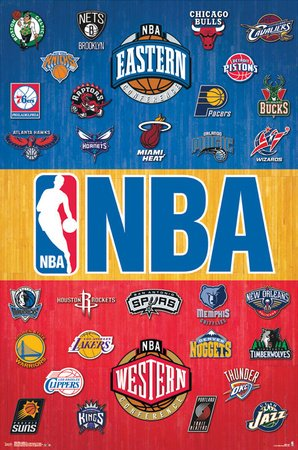
\includegraphics[height=280px]{eastandwest} \end{center}

The National Basketball Association (NBA) is one of the most worldwide
popular sporting events that is held every year in the world.

\begin{itemize}
\tightlist
\item
  It has two conferences, East and West, with 15 teams in each division.
\item
  30 teams fight in the league fight for a champion in a year-long
  season from October to June every year.
\item
  Each season is split into regular season and playoffs.
\item
  Each team has 82 matches to play in their regular season
\item
  Teams in the same conference would play more often than those.
\item
  Only the top 8 teams in each division are able to enter the playoffs
  of the season.
\item
  Ranks are determined ascending by a special statistic called Games
  Behind:

  \begin{itemize}
  \tightlist
  \item
    When team a is the leading team of the conference.
    \[Team B’s games behind=\frac {(Team A’s Wins-Team A’s Losses)-(Team B’s Wins-Team B’s Losses)}{2}\]
  \end{itemize}
\end{itemize}

Thus which 16 teams would enter the playoffs every season is one of the
biggest mystery in NBA every season.

Our goal, as introduced above, is simulating match results and
predicting NBA playoff teams. In other words, we are going to predict
which eight teams in each conference would get the lowest games behind
by the end of the regular season.

The focus is on the past 17-18 season. We will try to predict based on
prior part of this season's real data, and comparing our results with
this season's real data in the rest season to calculate our method's
accuracy. If we found our prediction is reliable in this season, we have
prepared data in the past 10 years for test and verification.

\hypertarget{methods}{%
\section{Methods}\label{methods}}

\hypertarget{processing-data}{%
\subsection{Processing Data}\label{processing-data}}

We made two tables A and B to store the standing data of all teams (in
A) and the match data of each matches (in B).

Then use the ``current'' standing data in A to simulate upcoming matches
in B and use the following match data to regenerate new standing data in
A

\begin{center}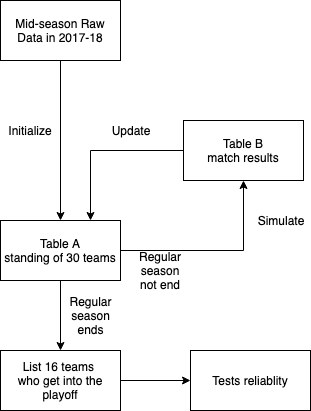
\includegraphics{methods_flowchart} \end{center}

Raw data used:

From 2017-18\_standing.csv

\begin{Shaded}
\begin{Highlighting}[]
\KeywordTok{str}\NormalTok{(standing_data[,}\KeywordTok{c}\NormalTok{(}\DecValTok{1}\NormalTok{,}\DecValTok{2}\NormalTok{,}\DecValTok{13}\NormalTok{,}\DecValTok{14}\NormalTok{,}\DecValTok{15}\NormalTok{,}\DecValTok{16}\NormalTok{,}\DecValTok{17}\NormalTok{,}\DecValTok{18}\NormalTok{,}\DecValTok{20}\NormalTok{,}\DecValTok{21}\NormalTok{)])}
\end{Highlighting}
\end{Shaded}

\begin{verbatim}
## 'data.frame':    5040 obs. of  10 variables:
##  $ stDate  : Factor w/ 168 levels "2017-10-17","2017-10-18",..: 1 1 1 1 1 1 1 1 1 1 ...
##  $ teamAbbr: Factor w/ 30 levels "ATL","BKN","BOS",..: 1 2 3 4 5 6 7 8 9 10 ...
##  $ homeWin : int  0 0 0 0 0 1 0 0 0 0 ...
##  $ homeLoss: int  0 0 0 0 0 0 0 0 0 1 ...
##  $ awayWin : int  0 0 0 0 0 0 0 0 0 0 ...
##  $ awayLoss: int  0 0 1 0 0 0 0 0 0 0 ...
##  $ confWin : int  0 0 0 0 0 1 0 0 0 0 ...
##  $ confLoss: int  0 0 1 0 0 0 0 0 0 1 ...
##  $ lastTen : int  0 0 0 0 0 1 0 0 0 0 ...
##  $ gamePlay: int  0 0 1 0 0 1 0 0 0 1 ...
\end{verbatim}

From 2017-18\_teamBoxScore.csv

\begin{Shaded}
\begin{Highlighting}[]
\KeywordTok{str}\NormalTok{(match_data[,}\KeywordTok{c}\NormalTok{(}\DecValTok{1}\NormalTok{,}\DecValTok{10}\NormalTok{,}\DecValTok{11}\NormalTok{,}\DecValTok{13}\NormalTok{,}\DecValTok{14}\NormalTok{,}\DecValTok{17}\NormalTok{,}\DecValTok{73}\NormalTok{)])}
\end{Highlighting}
\end{Shaded}

\begin{verbatim}
## 'data.frame':    2460 obs. of  7 variables:
##  $ gmDate  : Factor w/ 168 levels "2017-10-17","2017-10-18",..: 1 1 1 1 2 2 2 2 2 2 ...
##  $ teamAbbr: Factor w/ 30 levels "ATL","BKN","BOS",..: 3 6 11 10 4 9 2 12 16 22 ...
##  $ teamConf: Factor w/ 2 levels "East","West": 1 1 2 2 1 1 1 1 1 1 ...
##  $ teamLoc : Factor w/ 2 levels "Away","Home": 1 2 1 2 1 2 1 2 1 2 ...
##  $ teamRslt: Factor w/ 2 levels "Loss","Win": 1 2 2 1 1 2 1 2 1 2 ...
##  $ teamPTS : int  99 102 122 121 90 102 131 140 109 116 ...
##  $ opptPTS : int  102 99 121 122 102 90 140 131 116 109 ...
\end{verbatim}

Initial table A:

\begin{Shaded}
\begin{Highlighting}[]
\KeywordTok{str}\NormalTok{(tablea180311)}
\end{Highlighting}
\end{Shaded}

\begin{verbatim}
## 'data.frame':    30 obs. of  26 variables:
##  $ teamname     : Factor w/ 30 levels "ATL","BKN","BOS",..: 1 2 3 4 5 6 7 8 9 10 ...
##  $ confname     : Factor w/ 2 levels "East","West": 1 1 1 1 1 1 2 2 1 2 ...
##  $ homerate     : num  0.429 0.353 0.657 0.528 0.455 ...
##  $ awayrate     : num  0.156 0.273 0.719 0.323 0.242 ...
##  $ last10       : num  0.2 0.2 0.6 0.5 0.3 0.4 0.3 0.6 0.3 0.7 ...
##  $ homescorewin : num  105 105 104 108 103 ...
##  $ homescorelost: num  108.2 108.4 99.7 107.2 105.9 ...
##  $ awayscorewin : num  102 107 104 105 104 ...
##  $ awayscorelost: num  109 112 101 108 113 ...
##  $ confrate     : num  0.209 0.359 0.674 0.425 0.45 ...
##  $ numberdayoff : num  2 3 3 1 2 2 1 2 2 2 ...
##  $ lastgame     : Factor w/ 2 levels "Away","Home": 1 1 1 2 1 1 2 2 2 1 ...
##  $ totalmatch   : int  67 67 67 67 66 66 67 67 66 67 ...
##  $ confmatch    : int  43 39 43 40 40 41 45 45 45 41 ...
##  $ homematch    : int  35 34 35 36 33 33 36 36 35 33 ...
##  $ awaymatch    : int  32 33 32 31 33 33 31 31 31 34 ...
##  $ l1           : num  1 1 1 2 2 1 1 2 2 1 ...
##  $ l2           : num  1 2 2 1 1 1 2 2 1 1 ...
##  $ l3           : num  1 1 2 1 2 2 2 1 1 2 ...
##  $ l4           : num  2 1 1 1 1 2 1 1 1 2 ...
##  $ l5           : num  1 1 2 1 2 1 1 2 1 2 ...
##  $ l6           : num  2 1 2 1 1 1 1 2 2 2 ...
##  $ l7           : num  1 2 2 2 1 2 2 1 1 2 ...
##  $ l8           : num  1 1 2 2 1 1 1 1 1 2 ...
##  $ l9           : num  1 1 1 2 1 2 1 2 1 2 ...
##  $ l10          : num  1 1 1 2 1 1 1 2 2 1 ...
\end{verbatim}

Columns' meaning:

\begin{itemize}
\tightlist
\item
  ``Teamname'': Name of team
\item
  ``Confname'': East or West, which defines which conference the team
  belongs to.
\item
  ``Homerate'': winrate at home
\item
  ``Awayrate'': winrate away
\item
  ``Last10'': winrate in the last 10 matches
\item
  ``Homescorewin'': score won when at home
\item
  ``Homescorelost'': score lost when at home
\item
  ``Awayscorewin'': score win when playing away home
\item
  ``Awayscorelost'': score lost when to play away home
\item
  ``Confrate'': winrate when playing within the conference
\item
  ``Numberdayoff'': number of days since the last match
\item
  ``Lastgame'': is the last game played at home or away
\item
  ``totalmatch'':number of matches played
\item
  ``confmatch'':number of matches played within conference
\item
  ``Homematch'': number of matches played at home
\item
  ``Awaymatch'': number of matches played away
\item
  ``l1'' \textasciitilde{} ``l10'': is the last 1\textasciitilde{}10 win
  or lose
\end{itemize}

\hypertarget{generalized-linear-regression}{%
\subsection{Generalized Linear
Regression}\label{generalized-linear-regression}}

\hypertarget{permutation-test}{%
\subsection{Permutation Test}\label{permutation-test}}

The generalized linear model we used to predict the game result includes
predictors that might be correlated to each other. For example,
\texttt{homeTeamRate} and \texttt{homeTeamlast10} seem to be positively
correlated in common sense. Therefore, to improve our regression fit, we
want to thorougly examine the correlations among the variables and
proceed to use ridge regression if the variables are confirmed to be
correlated. The variables for testing are,

\begin{itemize}
\tightlist
\item
  homeTeamRate
\item
  awayTeamRate
\item
  homeTeamlast10
\item
  awayTeamlast10
\item
  histRate
\end{itemize}

A permutation test essentially checks if X and Y have the same
distribution by doing the following procedure,

\begin{enumerate}
\def\labelenumi{\arabic{enumi}.}
\tightlist
\item
  Observe a test statistic for the null hypothesis, \(H_0\)
\item
  For each replicated \(b = 1, 2,..., B\):

  \begin{itemize}
  \tightlist
  \item
    Generate a random permutation \(\pi\)
  \item
    Generate a new test statistic from the random permutation
  \end{itemize}
\item
  Get a Monte Carlo estimate of the p-value by calculating the
  probability of obtaining a new test statistic that is more extreme
  than the observed test statistic in the \(B\) replicates
\item
  Reject \(H_0\) at a significance level \(\alpha\) if the p-value is
  less than \(\alpha\).
\end{enumerate}

In our case, we can inherit the idea of permutation test and adapt it to
paired data to check the correlation in between. If there is truly no
association between X and Y, the distribution of \((X_i, Y_{\pi(i)})\)
will be the same as that of \((X_i, Y_i)\), where \(\pi(i)\) is the
\(i\)-th element of a permutation \(\pi\) of \({1, 2, ..., 13}\). We
implement this idea by randomly permuting Y and pairing it with a fixed
X and get a p-value for testing \(H_0: \rho = 0\) versus
\(H_1: \rho \neq 0\), where \(\rho\) is either the Pearson correlation
coefficient or the Spearman correlation coefficient:

\begin{itemize}
\item
  The \emph{Pearson Method} evaluates the \textbf{linear} relationship
  between two continuous variables, where a change in one variable is
  associated with a \textbf{proportional} change in the other variable.
\item
  The \emph{Spearman Method} is based on the ranked values for each
  variable rather than the raw data. It evaluates the \textbf{monotonic}
  relationship between two continuous or ordinal variables, where the
  variables tend to change together, but not necessarily at a constant
  rate. It is more general than the Pearson method.
\end{itemize}

To determine which correlation coefficient to use for which pair of
comparison, we plot variables against each another and added some noise
using \texttt{jitter()} to visualize the trend of relationship and
decide which method to use.

According to the plots, \emph{Home Rate vs.~Home Last 10}, \emph{Away
Rate vs.~Away Last 10}, \emph{Home Last 10 vs.~Historical Rate}, and
\emph{Away Last 10 vs.~Historical Rate} appear to be linear. We use the
Pearson method for these pairs. For the rest pairs, trends are not that
obvious. Therefore, we use the more genearl Spearman method.

\hypertarget{ridge-regression}{%
\subsection{Ridge Regression}\label{ridge-regression}}

\hypertarget{results}{%
\section{Results}\label{results}}

\hypertarget{linear-regrssion}{%
\subsection{Linear Regrssion}\label{linear-regrssion}}

\hypertarget{permutation-test-1}{%
\subsection{Permutation Test}\label{permutation-test-1}}

By performing permutation tests, we obtained the following table, which
shows all the pairs we tested, the method we used, the p-value for the
permutation test, and the decisions based on the p-values.

\begin{longtable}[]{@{}llll@{}}
\toprule
Pairs & Method & p-value & Decision\tabularnewline
\midrule
\endhead
Home Rate vs.~Home Last 10 & Pearson & 9.999e-05 &
Correlated\tabularnewline
Away Rate vs.~Away Last 10 & Pearson & 9.999e-05 &
Correlated\tabularnewline
Home Rate vs.~Historical Rate & Spearman & 9.999e-05 &
Correlated\tabularnewline
Away Rate vs.~Historical Rate & Spearman & 9.999e-05 &
Correlated\tabularnewline
Home Last 10 vs.~Historical Rate & Pearson & 9.999e-05 &
Correlated\tabularnewline
Away Last 10 vs.~Historical Rate & Pearson & 9.999e-05 &
Correlated\tabularnewline
Home Rate vs.~Away Rate & Spearman & 0.4131587 & Not
Correlated\tabularnewline
Home Last 10 vs.~Away Last 10 & Spearman & 9.999e-05 &
Correlated\tabularnewline
Home Rate vs.~Away Last 10 & Spearman & 0.02689731 &
Correlated\tabularnewline
Away Rate vs.~Home Last 10 & Spearman & 0.02329767 &
Correlated\tabularnewline
\bottomrule
\end{longtable}

We found that all pairs of variables have correlation except \emph{Home
Rate vs.~Away Rate}. This observation suggests that there exists problem
of collinearity among the predictors. It leads us to further examine the
VIF (Variance Inflation Factor) of the predictors and fit a Ridge
Regression model to remedy the problem of collinearity.

\hypertarget{ridge-regression-1}{%
\subsection{Ridge Regression}\label{ridge-regression-1}}

\hypertarget{discussion}{%
\section{Discussion}\label{discussion}}

The test for correlation is not very accurate because the ``Last 10''
data (i.e. \texttt{homeTeamlast10} and \texttt{awayTeamlast10}) are
highly categorical (discrete) because based on their calculation
criteria: the number of times the team wins, which is an integer,
divided by 10. When the ``Last 10'' data is paired with the other
continuous variables, such as \texttt{homeTeamRate} and
\texttt{histRate}, the correlation between a continuous variable and a
somewhat discrete variable cannot be simply determined by correlation
coefficients.

\newpage

\hypertarget{appendix}{%
\section{Appendix}\label{appendix}}

\hypertarget{scatterplots-for-correlation}{%
\subsubsection{Scatterplots for
Correlation}\label{scatterplots-for-correlation}}

\includegraphics{group6_written_report_files/figure-latex/unnamed-chunk-8-1.pdf}
\includegraphics{group6_written_report_files/figure-latex/unnamed-chunk-8-2.pdf}
\includegraphics{group6_written_report_files/figure-latex/unnamed-chunk-8-3.pdf}

\hypertarget{permutation-test-with-either-correlation-coefficient}{%
\subsubsection{Permutation Test with either correlation
coefficient}\label{permutation-test-with-either-correlation-coefficient}}

\begin{Shaded}
\begin{Highlighting}[]
\NormalTok{perm_test =}\StringTok{ }\ControlFlowTok{function}\NormalTok{(X, Y, }\DataTypeTok{B =} \DecValTok{10000}\NormalTok{, }\DataTypeTok{method =} \StringTok{"pearson"}\NormalTok{) \{}
\NormalTok{  nu =}\StringTok{ }\KeywordTok{seq_along}\NormalTok{(X)}
\NormalTok{  reps =}\StringTok{ }\KeywordTok{numeric}\NormalTok{(B)}
  
  \ControlFlowTok{if}\NormalTok{ (method }\OperatorTok{==}\StringTok{ "pearson"}\NormalTok{) \{ }\CommentTok{# Pearson Method - default}
\NormalTok{    rho0 =}\StringTok{ }\KeywordTok{abs}\NormalTok{(}\KeywordTok{cor}\NormalTok{(X, Y))}
    \ControlFlowTok{for}\NormalTok{ ( i }\ControlFlowTok{in} \DecValTok{1}\OperatorTok{:}\NormalTok{B ) \{}
\NormalTok{      perm =}\StringTok{ }\KeywordTok{sample}\NormalTok{(nu, }\DataTypeTok{size =} \KeywordTok{length}\NormalTok{(X), }\DataTypeTok{replace =} \OtherTok{FALSE}\NormalTok{)}
\NormalTok{      X1 =}\StringTok{ }\NormalTok{X[perm]}
\NormalTok{      reps[i] =}\StringTok{ }\KeywordTok{abs}\NormalTok{(}\KeywordTok{cor}\NormalTok{(X1, Y))}
\NormalTok{    \}}
\NormalTok{    pval =}\StringTok{ }\KeywordTok{mean}\NormalTok{(}\KeywordTok{c}\NormalTok{(rho0, reps) }\OperatorTok{>=}\StringTok{ }\NormalTok{rho0)}
\NormalTok{  \} }\ControlFlowTok{else} \ControlFlowTok{if}\NormalTok{ (method }\OperatorTok{==}\StringTok{ "spearman"}\NormalTok{) \{ }\CommentTok{# Spearman Method}
\NormalTok{    rho0 =}\StringTok{ }\KeywordTok{cor}\NormalTok{(X, Y, }\DataTypeTok{method =} \StringTok{"spearman"}\NormalTok{)}
\NormalTok{    t0 =}\StringTok{ }\KeywordTok{abs}\NormalTok{(rho0}\OperatorTok{*}\KeywordTok{sqrt}\NormalTok{((}\KeywordTok{length}\NormalTok{(X) }\OperatorTok{-}\StringTok{ }\DecValTok{2}\NormalTok{)}\OperatorTok{/}\NormalTok{(}\DecValTok{1} \OperatorTok{-}\StringTok{ }\NormalTok{rho0}\OperatorTok{^}\DecValTok{2}\NormalTok{)))}
    \ControlFlowTok{for}\NormalTok{ ( i }\ControlFlowTok{in} \DecValTok{1}\OperatorTok{:}\NormalTok{B ) \{}
\NormalTok{      perm =}\StringTok{ }\KeywordTok{sample}\NormalTok{(nu, }\DataTypeTok{size =} \KeywordTok{length}\NormalTok{(X), }\DataTypeTok{replace =} \OtherTok{FALSE}\NormalTok{)}
\NormalTok{      X1 =}\StringTok{ }\NormalTok{X[perm]}
\NormalTok{      rho =}\StringTok{ }\KeywordTok{cor}\NormalTok{(X1, Y, }\DataTypeTok{method =} \StringTok{"spearman"}\NormalTok{)}
\NormalTok{      reps[i] =}\StringTok{ }\KeywordTok{abs}\NormalTok{(rho}\OperatorTok{*}\KeywordTok{sqrt}\NormalTok{((}\KeywordTok{length}\NormalTok{(X) }\OperatorTok{-}\StringTok{ }\DecValTok{2}\NormalTok{)}\OperatorTok{/}\NormalTok{(}\DecValTok{1} \OperatorTok{-}\StringTok{ }\NormalTok{rho}\OperatorTok{^}\DecValTok{2}\NormalTok{)))}
\NormalTok{    \}}
\NormalTok{    pval =}\StringTok{ }\KeywordTok{mean}\NormalTok{(}\KeywordTok{c}\NormalTok{(t0, reps) }\OperatorTok{>=}\StringTok{ }\NormalTok{t0)}
\NormalTok{  \}}
  
  \KeywordTok{return}\NormalTok{(pval)}
\NormalTok{\}}

\CommentTok{# running the tests}
\KeywordTok{perm_test}\NormalTok{(data}\OperatorTok{$}\NormalTok{homeTeamRate, data}\OperatorTok{$}\NormalTok{homeTeamlast10, }\DecValTok{10000}\NormalTok{, }\StringTok{"pearson"}\NormalTok{)}
\KeywordTok{perm_test}\NormalTok{(data}\OperatorTok{$}\NormalTok{awayTeamRate, data}\OperatorTok{$}\NormalTok{awayTeamlast10, }\DecValTok{10000}\NormalTok{, }\StringTok{"pearson"}\NormalTok{)}
\KeywordTok{perm_test}\NormalTok{(data}\OperatorTok{$}\NormalTok{homeTeamRate, data}\OperatorTok{$}\NormalTok{histRate, }\DecValTok{10000}\NormalTok{, }\StringTok{"spearman"}\NormalTok{)}
\KeywordTok{perm_test}\NormalTok{(data}\OperatorTok{$}\NormalTok{awayTeamRate, data}\OperatorTok{$}\NormalTok{histRate, }\DecValTok{10000}\NormalTok{, }\StringTok{"spearman"}\NormalTok{)}
\KeywordTok{perm_test}\NormalTok{(data}\OperatorTok{$}\NormalTok{homeTeamlast10, data}\OperatorTok{$}\NormalTok{histRate, }\DecValTok{10000}\NormalTok{, }\StringTok{"spearman"}\NormalTok{)}
\KeywordTok{perm_test}\NormalTok{(data}\OperatorTok{$}\NormalTok{awayTeamlast10, data}\OperatorTok{$}\NormalTok{histRate, }\DecValTok{10000}\NormalTok{, }\StringTok{"spearman"}\NormalTok{)}
\KeywordTok{perm_test}\NormalTok{(data}\OperatorTok{$}\NormalTok{homeTeamRate, data}\OperatorTok{$}\NormalTok{awayTeamRate, }\DecValTok{10000}\NormalTok{, }\StringTok{"spearman"}\NormalTok{)}
\KeywordTok{perm_test}\NormalTok{(data}\OperatorTok{$}\NormalTok{homeTeamlast10, data}\OperatorTok{$}\NormalTok{awayTeamlast10, }\DecValTok{10000}\NormalTok{, }\StringTok{"spearman"}\NormalTok{)}
\KeywordTok{perm_test}\NormalTok{(data}\OperatorTok{$}\NormalTok{homeTeamRate, data}\OperatorTok{$}\NormalTok{awayTeamlast10, }\DecValTok{10000}\NormalTok{, }\StringTok{"spearman"}\NormalTok{)}
\KeywordTok{perm_test}\NormalTok{(data}\OperatorTok{$}\NormalTok{awayTeamRate, data}\OperatorTok{$}\NormalTok{homeTeamlast10, }\DecValTok{10000}\NormalTok{, }\StringTok{"spearman"}\NormalTok{)}
\end{Highlighting}
\end{Shaded}


\end{document}
